%TODO Formatting
\section{Das Leistungsportfolio im Ausbildungsbetrieb präsentieren}
\subsection{Arbeitsplätze und Arbeitsumgebungen für IT-Systeme beschreiben}
    \begin{subindent}
        IT ist heutzutage sowohl im privaten sowie industriellen Kontext nicht wegzudenken. \\
        Einsatzbereiche der IT\@:
    \end{subindent}
    
    \begin{itemize}[leftmargin=2.5cm, topsep=0.3em, itemsep=0.1em, parsep=0.5em]
        \item Privat
        \item Industrie
        \item Wirtschaft
        \item Verwaltung
    \end{itemize}
    
    \begin{subindent}
        Formen von Arbeitsarten:
    \end{subindent}
    
    \begin{itemize}[leftmargin=2.5cm, topsep=0.3em, itemsep=0.1em, parsep=0.5em]
        \item Telearbeiten: Arbeiten an einem eingerichteten Arbeitsplatz
        \item mobiles Arbeiten: auch Homeoffice, Arbeit nicht an festen Arbeitsplatz gebunden
    \end{itemize}
    
    \begin{subindent}
        Die Arbeitsplätze dieser Arten sind nach Bürokonzepten gestaltet und müssen ergonomische, ökologische und gesundheitliche Anforderungen berücksichtigen. \\
        Formen von Arbeitsumgebungen:
    \end{subindent}
    
    \begin{itemize}[leftmargin=2.5cm, topsep=0.3em, itemsep=0.1em, parsep=0.5em]
        \item Zellenbüros: Ein-/Mehrpersonenbüros entlang eines FLurs
        \item Großraumbüros: Open-Space-Bürolandschaft
        \item Kombibüro: Einzelbüros entlag der Fassade, Pausenraum dazwischen
        \item Non-Territoriales Büro: Büroplätze werden von Mitarbeitern für Arbeitszeit gebucht
    \end{itemize}
    
    \begin{subindent}
        Bei der Gestaltung der Arbeitsplätze muss auf genügend Beleuchtung (min. 500 Lux) sowie eine nicht zu hohe Lärmentwicklung (30-45dB) geachtet werden.
    \end{subindent}

\subsection{Marktgängige IT-Systeme vorstellen}
    \begin{tcolorbox}[width=15cm, center, title=Konfiguration, coltitle=white, colframe=orange, colback=white!60!orange]
        Bezeichnung für die Zusammenstellung, Einstellung und Abstimmung von Komponenten/Geräten/Programmen in Bezug auf Anwendung. \\
        Unterscheidung vom Istzustand (Ist-Konfiguration) als aktuellem Stand und Sollzustand (Soll-Konfiguration) als Zielzustand.
    \end{tcolorbox}
    %TODO evtl die verschiedenen bauformen adden
    \vspace{-1em}
    
    \begin{figure}[h]
        \centering
        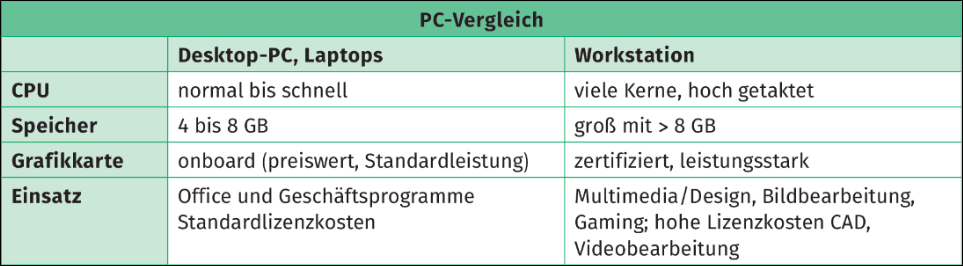
\includegraphics[width=0.7\textwidth]{./images/2.2.2_pc-vergleich.png}
        \caption{Unterscheidung der Leistungsfähigkeit}\label{fig:Leistungsfähigkeit_Unterscheidung}
    \end{figure}
    
    \begin{subindent}
        IT-Hardware kann auf verschiedene Kriterien und Spezifikationen geprüft werden. \\
        Dabei sind die folgenden von besonderer Bedeutung:
    \end{subindent}
    
    \begin{itemize}[leftmargin=2.5cm, topsep=0.3em, itemsep=0.1em, parsep=0.5em]
        \item Quantitative Größen (messbare, objektive Größen)
        \item Qualitative Größen (schwer messbare, subjektive Größen)
        \item Vergleiche (Stress-/Benchmarktests, etc.)
    \end{itemize}
    
    \begin{subindent}
        Desweiteren können zusätzliche Recherchen durchgeführt werden, etwa über das Internet (Fachportale, Blogs, etc.) oder Hardware-Tests und Diagnosetools.
    
    \end{subindent}

\subsection{Das Leistungsportfolio im IT-Bereich präsentieren}
    \begin{subindent}
        Das Leistungsportfolio eines Unternehmens beschreibt die Dientsleistungen und Tätigkeiten eines Betriebs. \\
        Bei Unternehmen mit interner IT, ist die IT-Abteilung der Dienstleister der Mitarbeiter und Abteilungen. Die Mitarbeiter sind demnach interne Kunden.
    \end{subindent}

\subsection*{Reflexion Kapitel 2.2}
\addcontentsline{toc}{subsection}{Reflexion Kapitel 2.2}
    %TODO REFLEXION
    \begin{refindent}
        TODO
    \end{refindent}